\acused{KNN}
\label{chap:KNNs}
Durch künstliche neuronale Netze (\acsp{KNN}) können Maschinen lernen, bestimmte Probleme zu lösen, ohne dass ein Mensch vorher explizite Regeln dafür definieren muss. Dies steht im Kontrast zur Methode, der Maschine  vorher einen festen, vollständigen Regelsatz bereitzustellen. Letztgenannter Ansatz zeigt in einigen Gebieten nur begrenzten Erfolg, da es für Menschen herausfordernd sein kann, Regelsätze für Vorgänge zu definieren, die unbewusst im Gehirn stattfinden oder viel Kontext erfordern. Zu nennen sind hierbei die visuelle Objekterkennung oder menschliche Sprache. Außerdem können neue, nicht in den Regeln beachtete Situationen dazu führen, dass die Maschine das Problem nicht mehr lösen kann. Die Grundidee hinter \acp{KNN} ist deshalb, dass sich die Maschine selber einen Wissensschatz aufbaut, der ihr beim Lösen des Problems hilft. Dies geschieht, indem die Entwickler ihr reale Trainingsbeispiele zeigen. Möchte man einen Algorithmus trainieren, der Schach spielen soll, kann man ihm beispielsweise eine Vielzahl an realen Schachpartien zeigen. Anhand dessen lernt der Algorithmus verschiedene Strategien und baut ein Spielverständnis auf, das womöglich über die menschlichen Fähigkeiten hinausgeht. \cite[S. 1ff.]{DeepLearningBook}

In den letzten Jahrzehnten erlebte das maschinelle Lernen und damit auch das Gebiet der \acp{KNN} einen Aufschwung. Es existiert bereits seit Mitte des vergangenen Jarhunderts, wird allerdings erst durch die zunehmende Rechenleistung und die Verfügbarkeit von großen Datenmengen flächendeckend eingesetzt. Einsatzgebiete für \acp{KNN} sind unter anderem die Objekterkennung, das Verstehen von natürlicher Sprache und die Generierung von Text und Bildern. \cite[S. 4,17]{knnsKompakt}

Die Inspiration für \acp{KNN} bildet die Informationsverarbeitung des Gehirns in Lebewesen. Die kleinste hier betrachtete Einheit ist das Neuron. Neuronen in \acp{KNN} sind konzeptionell inspiriert von realen, biologischen Neuronen, besitzen aber eine deutlich abstrahierte Funktionsweise. In \acp{KNN} berechnen sie ein Skalarprodukt ihrer gewichteten Eingangswerte, addieren einen sogennaten \emph{Bias} hinzu und wenden auf das Ergebnis eine nichtlineare Funktion an. Letzere wird auch als Aktivierungsfunktion bezeichnet. Diese Aktivierungsfunktion kann analog dazu gesehen werden, dass biologische Neuronen einen Schwellenwert (\emph{engl.: threshold}) besitzen, der überschritten werden muss, damit das Neuron \emph{feuert}, also einen Impuls an weitere Neuronen weitergibt. Aktivierungsfunktionen sind notwendig, damit neuronale Netze Probleme lösen können, die über die Fähigkeiten einer linearen Regression hinausgehen. Es wird eine nichtlineare Abhängigkeit zwischen dem Eingang $X$ und dem Ausgang $Y$ umgesetzt. \cite{visualApproach}

In der Nachfolgenden Abbildung ist ein einzelnes künstliches Neuron eines \acp{KNN} darstellt. Das \emph{Plus-Zeichen} steht für die Berechnung des Skalarprodukts der Eingänge und der darauf addierte Bias. Die Aktivierungsfunktion wird durch das \emph{Sigmoid}-Zeichen simbolisiert. Der Ausgang (\emph{rechts}) ist das Ergebnis der Berechnung des Neurons. \cite{visualApproach}

\begin{figure}[H]
   \centering
   \includegraphics[width=0.4\textwidth]{images/KNNs/Neuron.png}
   \caption{Einzelnes Neuron eines \acp{KNN} \cite{visualApproach}}
\end{figure}

Um komplexe Probleme lösen zu können, werden mehre Neuronen miteinander verbunden und in Schichten angeordnet. Jede Schicht erhält die Ausgangswerte der vorherigen Schicht als Eingang und gibt die daraus berechneten, neuen Werte an die nächste Schicht weiter. Abbildung \ref{fig:KNN} zeigt ein vollständiges \ac{KNN}. Die Neuronen sind durch Kreise dargestellt und ihre Verbindungen durch Linien. \cite{knnsKompakt} 

\begin{figure}[H]
   \centering
   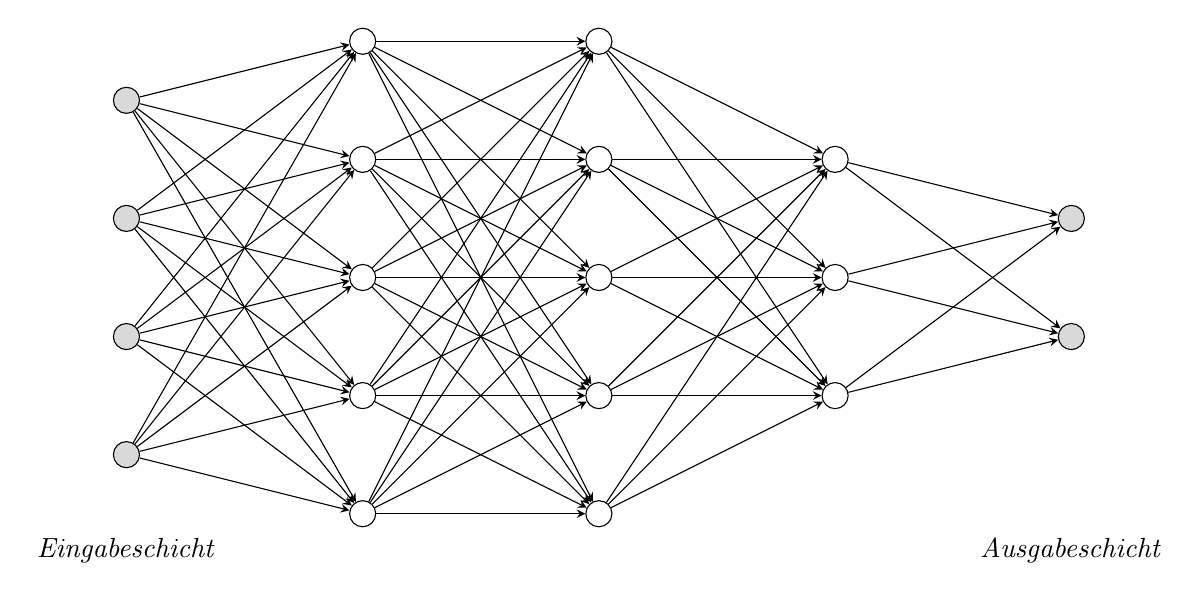
\begin{tikzpicture}[x=1.5cm, y=1.5cm, >=stealth]
      % Input layer
      \foreach \i in {1,...,4}
      \node[circle, draw=black, fill=gray!30] (in-\i) at (0,\i-2) {};
      
      % Hidden layer 1
      \foreach \i in {1,...,5}
      \node[circle, draw=black, fill=white] (h1-\i) at (2,\i-2.5) {};
      
      % Hidden layer 2
      \foreach \i in {1,...,5}
      \node[circle, draw=black, fill=white] (h2-\i) at (4,\i-2.5) {};

      % Hidden layer 3
      \foreach \i in {1,...,3}
      \node[circle, draw=black, fill=white] (h3-\i) at (6, \i-1.5) {};
      
      % Output layer
      \foreach \i in {1,...,2}
      \node[circle, draw=black, fill=gray!30] (out-\i) at (8,\i-1) {};
      
      % Connections
      \foreach \i in {1,...,4}
      \foreach \j in {1,...,5}
      \draw[->] (in-\i) -- (h1-\j);
      
      \foreach \i in {1,...,5}
      \foreach \j in {1,...,5}
      \draw[->] (h1-\i) -- (h2-\j);

      \foreach \i in {1,...,5}
      \foreach \j in {1,...,3}
      \draw[->] (h2-\i) -- (h3-\j);
      
      \foreach \i in {1,...,3}
      \foreach \j in {1,...,2}
      \draw[->] (h3-\i) -- (out-\j);
      
      % Labels
      \node[above] at (0,-2) {\emph{Eingabeschicht}};
      \node[above] at (8,-2) {\emph{Ausgabeschicht}};
      
   \end{tikzpicture}
		\caption{Vollständiges \ac{KNN} \emph{(angelehnt an \cite{visualApproach})}}
      \label{fig:KNN}
\end{figure}

Eine Verbindung stellt dar, dass ein Neuron seinen berechneten Wert an das nachfolgende Neuron weitergibt. Dies geschieht hierbei ausschließlich von \emph{links nach rechts}, womit das \ac{KNN} als \emph{Feedforward-Netzwerk} bezeichnet wird. Die Eingabeschicht erhält die Eingabewerte des Netzwerks, die Ausgabeschicht liefert die Vorhersage des Modells. Zwischen diesen beiden Schichten befinden sich beliebig viele verarbeitende Schichten, die als \emph{Hidden Layer} bezeichnet werden. \cite{knnsKompakt}

Die Vorhersage, gekennzeichnet durch die Werte der Ausgabeschicht, hängt von den jeweiligen Parametern der Neuronen des Netzwerks ab. Dies sind die Gewichte (\emph{engl.: weights}) der Verbindungen zwischen den Neuronen sowie der Bias der Neuronen. Es existieren auch trainierbare Aktivierungsfunktionen, diese sind jedoch vergleichsweise unüblich. Entwickler sind für den Entwurf der Netzwerkarchitektur zuständig, die Parameter werden jedoch durch das Modell trainiert. Zu Beginn besitzt das Modell zufällige Parameter, wodurch es in der Regel nicht die gewünschte Abbildung zwischen Ein- und Ausgabe implementiert. Ein untrainierter Schachalgorithmus spielt demnach augenscheinlich willkürliche Züge. Ein untrainierter Katzenklassifikator besitzt keinen erkennbaren Wissensschatz darüber, welche Charakteristiken eine Katze optisch auszeichnen. Das Ziel des Trainings ist, dass die Parameter des Modells zunehmend gegen das Optimum konvergieren und so das Modell immer plausibler in seinen Vorhersagen wird. \cite{knnsKompakt} \cite{visualApproach}

%---------------------------------------------------------------------------------------------------------------
\subsection{Training}
Für das Training von \acp{KNN} werden Daten benötigt. Zum einen ein Satz an \emph{Trainingsdaten} und zum anderen ein Satz an \emph{Testdaten}. Die Trainingsdaten dienen dazu, das Modell zu verbessern. Eine \emph{Kostenfunktion} berechnet, wie genau die Vorhersagen des Modells auf den Trainingsdaten sind. Darauf basierend wird das Modell optimiert. Die Testdaten dienen zur Messung der Qualität des Modells. Es kann nämlich vorkommen, dass das \ac{KNN} die Trainingsdaten \emph{auswendig} lernt und deshalb hier gute Ergebnisse erzielt, aber eine unzureichende Performanz auf den Testdaten zeigt. Etwa wenn das \ac{KNN} unerwartete Eigenschaften in den Trainingsdaten lernt. Aus diesem Grund werden trainierte Modelle nur anhand der Testdaten evaluiert. \cite{knnsKompakt}

Die Kostenfunktion bestimmt die durchschnittliche Fehlerrate des \acp{KNN} auf einem gegebenen Datensatz. Sie berechnet somit, gemittelt über alle $m$ Beispiele aus dem Datensatz, die Abweichung des vorhergesagten Wertes $\hat{y}$ von dem tatsächlichen Wert $y$. Für ein einzelnes Beispiel aus dem Datensatz nutzt die Funktion dafür eine \emph{Verlustfunktion} $\mathcal{L}$. Die Verlustfunktion bewertet somit eine einzelne Aussage des \ac{KNN}, während die Kostenfunktion die durchschnittliche Qualität der Aussagen auf dem gesamten Datensatz misst. Folgende Gleichung zeigt die Kostenfunktion: \cite{DeepLearningBook}

\begin{equation}
   \label{eq:costFunctionGeneral}
   J(\theta) = \frac{1}{m} \sum_{i=1}^{m} \mathcal{L}(\hat{y}^{(i)}, y^{(i)})
\end{equation}
Wobei: \newline
\emph{\null\quad\quad $J$: Wert der Kostenfunktion \newline
\null\quad\quad $\theta$: Trainierbare Parameter des Modells \newline
\null\quad\quad $m$: Anzahl der Trainingsbeispiele \newline
\null\quad\quad $i$: Index des momentan betrachteten Trainingsbeispiels \newline
\null\quad\quad $\mathcal{L}$: Verlustfunktion \newline
\null\quad\quad $\hat{y}$: Vorhersage des Modells \newline
\null\quad\quad $y$: Erwarteter Wert}

Die Kostenfunktion $J$ ist abhängig von einem $\theta$. Das $\theta$ ist ein Vektor, der alle Gewichte und Biases und damit alle trainierbaren Parameter des \acp{KNN} beinhaltet. Verändern sich die Parameter des \acp{KNN}, dann liefert es andere Aussagen für das $\hat{y}$. Somit ändert sich der Wert der Kostenfunktion, wenn das \ac{KNN} seine Parameter anpasst.  \cite{DeepLearningBook}

Die Gleichung \ref{eq:costFunctionGeneral} kann auch mit dem Operator $\mathbb{E}$ formuliert werden. Er beschreibt den Erwartungswert: \cite{DeepLearningBook}
\begin{equation}
	\label{eq:costFunctionExpectedValue}
	J(\theta) = \mathbb{E}_{x,y}[\mathcal{L}(f(x; \theta), y)]
\end{equation}
Was in Gleichung \ref{eq:costFunctionGeneral} das arithmetische Mittel der Verlustfunktionen ist, wird hier als Erwartungswert der Verlustfunktion geschrieben. Die Fragestellung lautet: \emph{Wenn ein zufälliges Beispiel $x$ und das zugehörige $y$ aus dem Datensatz gezogen werden, was ist dann der erwartete Verlust des Modells?} Die Vorhersage $\hat{y}$ des \ac{KNN} wird hier als $f(x; \theta)$ geschrieben. Dabei ist $f$ das \ac{KNN}, das für ein gezogenes $x$ eine bestimmte Vorhersage trifft. Diese Vorhersage ist zudem abhängig von $\theta$. Diese alternative Darstellung der Kostenfunktion mit dem Operator $\mathbb{E}$ ist relevant für Kapitel \ref{chap:NoGANs}. \cite{DeepLearningBook}

Kostenfunktionen können verschiedene Arten von Verlustfunktionen verwenden. Für diese Arbeit sind sowohl die $\mathcal{L}_1$ und $\mathcal{L}_2$ Verlustfunktionen als auch der \emph{Binary Crossentropy Loss} von besonderer Relevanz.

\paragraph{$\mathcal{L}_1$ Verlustfunktion} Die $\mathcal{L}_1$ Verlustfunktion berechnet für ein gegebenes Beispiel die absolute Abweichung der Vorhersage von dem erwarteten Wert. Sie wird auch als \emph{mittlere absolute Abweichung} \emph{(engl.: mean absolute error)} bezeichnet.
\begin{equation}
   \mathcal{L}_1 = |\hat{y} - y|
\end{equation}

\paragraph{$\mathcal{L}_2$ Verlustfunktion} Die $\mathcal{L}_2$ Verlustfunktion berechnet hingegen die quadratische Abweichung von dem erwarteten Wert. Hier haben somit größe Abweichungen einen stärkeren Einfluss auf den \emph{Verlust} \emph{(eng.: loss)} als bei der $\mathcal{L}_1$ Funktion. Diese Verlustfunktion wird auch als \emph{mittlere quadratische Abweichung} \emph{(engl.: mean squared error)} bezeichnet.
\begin{equation}
   \mathcal{L}_2 = (\hat{y} - y)^2
\end{equation}

\paragraph{Binary Crossentropy Loss} Die Binary Crossentropy Verlustfunktion ist auch als \emph{logarithmische Verlustfunktion} bekannt. Sie eignet sich für binäre Klassifikationen, wo demnach das \ac{KNN} eine Wahrscheinlichkeit zwischen $0$ und $1$ ausgibt. Ein Beispiel hierfür ist, wenn das \ac{KNN} abschätzen soll, ob auf einem Bild eine Katze zu sehen ist oder nicht. Ein Schwellenwert für eine Wahrscheinlichkeit zwischen $0$ und $1$ gibt dann an, ob das Ergebnis als \emph{Ja} oder \emph{Nein} interpretiert wird. Die Binary Crossentropy Verlustfunktion ist in Gleichung \ref{eq:bce-loss} dargestellt. Wenn der erwartete Wert $y$ gleich $1$ ist, dann reduziert sich die Verlustfunktion zu $\mathcal{L} = -\log(\hat{y})$. Ist der erwartete Wert $y$ gleich $0$, dann reduziert sich die Verlustfunktion zu $\mathcal{L} = -\log(1 - \hat{y})$. Die Verlustfunktion nutzt die Eigenschaften aus, dass $\log(1) = 0$ ist und der Logarithmus von Werten zwischen $0$ und $1$ negativ ist. \cite{bce-loss}
\begin{equation}
	\label{eq:bce-loss}
   \mathcal{L}_{BCE} =  - [y \log(\hat{y}) + (1 - y) \log(1 - \hat{y})]
\end{equation}

Das Training des Modells besteht nicht nur daraus, die Vorhersagen des Modells zu bewerten. Damit das Modell in dem nächsten Trainingsdurchlauf idealerweise einen geringeren Wert für die Kostenfunktion erreicht, müssen die trainierbaren Parameter $\theta$ des Modells angepasst werden. Von ihnen hängt der Wert der Kostenfunktion ab. Die Ausgangssituation ist hierbei folgende: Mit einem gegebenen $\theta$ befindet sich das \ac{KNN} in einem bestimmten Punkt der Kostenfunktion $J(\theta)$. Gesucht ist eine Parameteränderung $\dif\theta$, mit der sich das \ac{KNN} am weitesten an das globale Minimum der Kostenfunktion annähert. Das globale Minimum ist die beste Lösung, die das Modell für die gegebenen Trainingsdaten finden kann und damit das Optimum. Da $J(\theta)$ eine viel-dimensionale Funktion ist, berechnet die Trainingsfunktion diesen Idealwert für $\theta$ nicht numerisch. Stattdessen nähert sich das \ac{KNN} mit jedem Trainingsschritt dem Optimum an. \cite{knnsKompakt}

Nähern tut sich das \ac{KNN} dem Optimum, indem es den Punkt $\theta$ in Richtung des negativen Gradienten der Kostenfunktion bewegt. Also die Richtung, in die, aus der momentanen Ausgangsposition, die Kostenfunktion den steilsten Abstieg besitzt. Pro Trainingsiteration bewegen sich die Parameter $\theta$ nur um einen kleinen Betrag in Richtung des negativen Gradienten. Das wird so lange durchgeführt, bis der Gradient einen so geringen Betrag hat, dass sich die Parameter des \ac{KNN} nicht mehr signifikant verändern. Das \ac{KNN} befindet sich hier bestenfalls im globalen Optimum. Der Betrag der Annäherung pro Trainingsschritt ist durch eine sogennante Lernrate $\alpha$ bestimmt. Die Lernrate ist ein \emph{Hyperparameter}, und damit klassischerweise ein nicht-trainierbarer Parameter, da sie durch die Entwickler fest bestimmt wird und nicht durch das Modell selbst gelernt wird. \cite{knnsKompakt}

\todo[inline]{Auf Ableitung der Kostenfunktion für Berechnung des Gradienten eingehen?}
\todo[inline]{Hier schon Batches erklären und damit darauf eingehen wie mit einer Verlustfunktion über mehrere Trainingsbeispiele trainiert wird}

%---------------------------------------------------------------------------------------------------------------
\subsection{Convolutional Neural Networks}
\acp{KNN} bewähren sich mitunter besonders im Bereich \emph{Computer Vision}. Ein Bereich, der sich mit der Interpretation von Bild- und Videodaten beschäftigt. Hier spielt die Mustererkennung eine tragende Rolle. Es sollen Merkmale erkannt werden, die jedes Objekt eines bestimmten Typs auszeichnen, die jedoch nicht auf jedem Bild die exakt identischen Pixelwerte besitzen. Die typische Form von Katzenohren ist beispielsweise ein Muster, das bei der Katzenerkennung verwendet werden kann. Es ist nicht trivial, allgemeine Regeln zu definieren, welche Pixelmuster als Katzenohr erkannt werden sollen und welche nicht. Deshalb wird hier auf \acp{KNN} zurückgegriffen.

Verwendet man hierfür jedoch die bisher beschriebene Netzwerkarchitektur, treten verschiedene Probleme auf. Jedes sogenannte \emph{Feature} des Eingangs wird über die Eingangsschicht in das \ac{KNN} gespeist. Bei einem Schachalgorithmus kann die Menge aller Features beispielsweise durch die momentane Position aller Figuren auf dem Schachbrett beschrieben werden. Das liegt daran, dass genau diese Werte den Ausgang des Netzwerks beeinflussen. In diesem Fall, welchen Zug der Algorithmus als nächstes spielt. Bei der Bildklassifizierung ist jeder Pixel des Bildes ein Feature. Ein Netz, das Bilder der Größe 1024x1024 Pixel mit drei Farbkanälen (rot, grün blau) klassifizieren soll, muss demnach folgende Anzahl an Eingängen verarbeiten:

\begin{equation}
   1024 \cdot 1024 \cdot 3 = 3.145.728
\end{equation}

Um eine derartige Anzahl an Eingängen sinnvoll interpretieren zu können, ist ein Netzwerk mit vielen Schichten und Neuronen notwendig. So vielen, dass auch heutige Computer an die grenzen ihrer Rechenleistung gelangen. Mitunter deshalb wird im Bereich Computer Vision auf \acp{CNN} zurückgegriffen. 

\acp{CNN} basieren auf der Faltung (engl.: convolution) einer Eingangsmatrix mit einer Faltmatrix. Jedes \ac{CNN} besitzt mindestens eine Schicht, die eine Faltung durchführt. Dabei schiebt das \ac{CNN} die Faltmatrix nach und nach über die Eingangsmatrix. Bei jedem Schritt berechnet es dabei das Skalarprodukt der momentan betrachteten Werte der Eingangsmatrix mit den Parametern der Faltmatrix. Das Ergebnis hiervon ist eine neue Matrix, die weniger Werte beinhaltet als der Eingang des \ac{CNN}. Folgt hierauf eine weitere Schicht, dann erhält sie das Ergebnis der Faltung als Eingabewert und nutzt eine eigene Faltmatrix um erneut eine Faltung durchzuführen. Die trainierbaren Parameter sind dabei die Werte der Faltmatrizen aller Schichten. Nachfolgende Abbildung soll die Faltung visualisieren:

\begin{figure}[H]
      \centering
      \includegraphics[width=0.8\textwidth]{images/KNNs/CNN Convolution.png}
      \caption{Beispiel für eine Faltung (engl.: Convolution) \cite{cnnsIntroduction}}
      \label{fig:convolution}
\end{figure}

Zunächst wird die Faltmatrix beispielsweise \emph{links oben} auf der Eingangsmatrix angewendet. Der betrachtete Teil der Eingangsmatrix wird hier als \emph{Pooled Vector} bezeichnet. Hierauf wird der Kernel, in diesem Fall ein sogenannter \emph{3x3-Kernel}, angewendet. Es wird also das Skalarprodukt der Werte mit dem gleichen Index aus dem \emph{Pooled Vector} und dem Kernel berechnet. In diesem Fall:
